\chapter{Estado del Arte}

A la fecha de realización de este estudio no existen trabajos que presenten como objetivo final la clasificación no supervisada de establecimientos educacionales y los alumnos matriculados en cada uno de ellos. Debido a esto se investigó sobre trabajos anteriores en el ámbito de la educación, en específico la elección de colegios, para así tener una guía de que variables son relevantes de considerar.

En el 2002 Sapelli y Torche \cite{SAPELLI2002} estudiaron los diferentes determinantes que inciden en la elección del tipo de colegio que realizan los padres al momento de matricular a sus hijos en un determinado establecimiento educacional. En este suponen que una mayor educación de los hijos proveerá a los padres  una probabilidad mayor de apoyo cuando estén en la vejez, por lo cual utilizan un modelo en donde se postula una función de utilidad para los padres. Dicha función depende del capital humano inicial de los hijos, el cual puede incrementarse con la educación, y del nivel de consumo presente. Para esto utilizaron diferentes fuentes de información, siendo las más relevantes la encuesta de caracterización socioeconómica (CASEN) de 1996 \cite{CASEN1996} y los resultados del SIMCE, en donde solo consideraron los datos referentes a la elección de establecimientos de enseñanza básica (niños entre 7 y 14 años), en donde el nivel de cobertura es cercano al 100\%\footnote{98,2\% de cobertura educacional para el nivel de enseñanza básica en el año 1996. Fuente: CASEN 1996.} y se descarta la opción de no elegir un colegio. Los factores más determinantes son el nivel de ingreso, la educación de los padres, la recepción de subsidios y la calidad del colegio. Los subsidios por colegios y no por alumno, es decir no son portables, dificultan el acceso a los colegios con menores subsidios para las familias de menores recursos. Otro punto importante que destacan es la alta sensibilidad que los padres demuestran respecto a la calidad de los colegios, aún sin conocer los resultados SIMCE, actúan de tal forma que hace pensar que los conocieran.

En el año 2009 Gallego y Hernando \cite{gallego2010school} buscando resolver la interrogante de cómo los padres escogen el colegio para sus hijos mejorando un modelo desarrollado anteriormente. Para el estudio se consideraron diferentes variables, las cuales se pueden agrupar en dos grandes categorías: características del alumno y características del colegio. En ambos casos los datos son obtenidos del SIMCE del 2012 o calculados por los autores a partir de dichos datos para un universo de 70.000 alumnos de cuarto básico que asisten a 1.200 colegios. Las dos variables que afectan más la elección de un colegio, son el resultado del establecimiento en las pruebas y la distancia entre el hogar y el colegio, en donde la primera variable se repite respecto al estudio \cite{SAPELLI2002}.

Dos años después, en el 2011, Daniel Gómez en conjunto con R. Chumacero y R. Paredes \cite{Chumacero20111103} realizan un estudio similar a los ya presentados, en donde consideran diversos factores que consideran los padres al escoger un determinado colegio. Dichos factores se pueden clasificar en características particulares de cada niño, las propias de cada establecimiento y las que asocian al niño con la escuela, como la distancia entre el hogar y el colegio. Para llevar a cabo esto establecieron una función similar a la presentada en \cite{SAPELLI2002}, donde se mide la utilidad de que un niño asista a un determinado colegio y que depende de los tres grupos de factores mencionados. Al igual que en trabajos anteriores fueron considerados datos de la encuesta CASEN y del SIMCE, ambos correspondientes al año 2003. Mediantes los estudios realizados llegaron a la conclusión de que de los factores analizados, la localización, el precio, la calidad y la potencial competencia de los establecimientos son determinantes al momento de realizar la elección, pero los más valorados por los padres son la calidad y la distancia.

Al año siguiente Gómez, Chumacero y Paredes \cite{GOMEZ2012}, buscan determinar si el conocimiento de resultados de pruebas específicas (SIMCE) determina de manera importante la selección que realizan los padres sobre el colegio donde matricular a sus hijos. Para esto realizaron un estudio comparativo, tomando como base el estudio anterior y comparándolo con datos de 1996 (primer año donde se hicieron públicos los resultados del SIMCE, por lo cual no influyen en la elección de colegios de ese año). Del estudio se obtuvo que aún sin conocer los resultados los padres actúan como si los conocieran escogiendo escuelas de mayor calidad, tal como se obtuvo en \cite{SAPELLI2002}. Además, cuando los resultados de las pruebas se hicieron públicos, este pasó a ser un factor aún más determinante al momento de tomar una decisión.

Finalmente, uno de los trabajos más recientes en torno a la selección de colegios fue realizado por Canales, Bellei y Orellana \cite{canalesque}, donde a diferencia de los trabajos anteriormente señalados, este se enfoca en un sector social específico para determinar y comprender el sentido que tiene para los padres de clase media el elegir un colegio privado. Para este estudio utilizaron dos técnicas complementarias: grupo de discusión y entrevista focalizada, donde la primera apunta a conocer cuál es el valor o significado colectivo de la decisión y la segunda permite conocer como el sujeto entiende la decisión que esta tomando. Los resultados obtenidos son de un carácter preocupante, ya que la selección de colegios esta guiada por el interés del sector medio de distanciarse y diferenciarse de los más pobres, siendo esto una decisión netamente clasista. Además esta preocupa del lado de la educación, debido a que al parecer ni familias ni escuelas parecen orientadas a mejorar el nivel de educación.

Sumado a los trabajos anteriormente señalados es importante conocer algunos conceptos que serán clave para el estudio.

\section{Machine Learning}

El \textit{Machine Learning} \cite{IBMML} o aprendizaje automático es una subrama de la inteligencia artificial que permite a un sistema aprender a través de los datos y no mediante una programación explícita. Este usa diferentes algoritmos que de manera iterativa aprenden de los datos, logrando mejorar la descripción de los datos y la predicción de resultados. Dichos algoritmos operan mediante la construcción de un modelo basado en conjuntos de datos de entrenamiento, que al ir iterando va consiguiendo modelos más precisos. Finalmente se obtiene un modelo de aprendizaje automático que es la salida generada al entrenar un algoritmo de aprendizaje con datos.

En otras palabras es una ciencia que permite el estudio del comportamiento o patrones presentes en diversos tipos de datos, para poder automatizar diversos procesos. Además esto implica un aprendizaje continuo que va mejorando con cada iteración haciéndolo más inteligente y capaz de resolver diferentes problemas en base a lo que va aprendiendo.

Su utilización en diversos ámbitos tiene variadas ventajas, esta permite mejorar la gestión organizacional, facilitar la toma de diferentes decisiones, automatizar y acelerar procesos, entre muchas otras. Pero como es de esperarse también presenta desventajas, las cuales vienen muy de la mano con las decisiones humanas, ya que estas decisiones afectan la resolución que toma el algoritmo en las tareas que se le asignan. Una mala decisión humana puede influir en malos resultados del algoritmo y un mal desempeño en las tareas asignadas.

Este aprendizaje se divide en dos: supervisado y no supervisado.

El aprendizaje supervisado consiste en intentar deducir a partir de datos de entrenamiento o ejemplo una función que clasifique datos sin una clasificación previa. En este caso los datos están compuestos por dos partes, por un lado están los diferentes atributos, ya sean numéricos o categóricos, y por otro lado una etiqueta que clasifica el dato. Entonces lo que se hace es determinar mediante los diferentes atributos el valor de la etiqueta, para luego poder predecir la clasificación de datos no categorizados. Un ejemplo de algoritmo de aprendizaje no supervisado es el de \textit{K} vecinos mas cercanos.

El aprendizaje no supervisado, a diferencia del supervisado no posee un conocimiento a priori de una clasificación de los datos. Por lo tanto un modelo se ajusta al número de observaciones que contiene un data set. En este tipo de aprendizaje solo se cuenta con diferentes atributos, sobre los cuales se buscan semejanzas para poder clasificarlos y crear agrupaciones o clústers. Algunos ejemplos de algoritmos de aprendizaje no supervisado son K-Means y la extensión propuesta en \cite{Pelleg00x-means:extending}, X-Means.

\section{Clustering}

El agrupamiento o \textit{clustering} \cite{clusteranalysis} es un procedimiento que consiste en buscar grupos en un conjunto de datos, estos se denominan clústers y encontrarlos es el objetivo principal del análisis de clústers. Lo que se busca con esto es básicamente formar grupos que contengan objetos similares entre sí y que sean lo más diferente posible con los objetos de otros grupos.

Esta tarea es una actividad importante del proceso de aprendizaje del ser humano, la cual comienza desde muy pequeños. Tareas como la distinción entre perros y gatos u hombres y mujeres, entre muchos otros, son claros ejemplos de esto. La clasificación siempre a jugado un papel muy importante dentro de la ciencia y es por esto que existen innumerables aplicaciones, tales como la clasificación de compuesto en química, la identificación de diversas enfermedades en la medicina, la clasificación de estrellas en la astronomía, etc.

\begin{figure}[H]
    \centering
    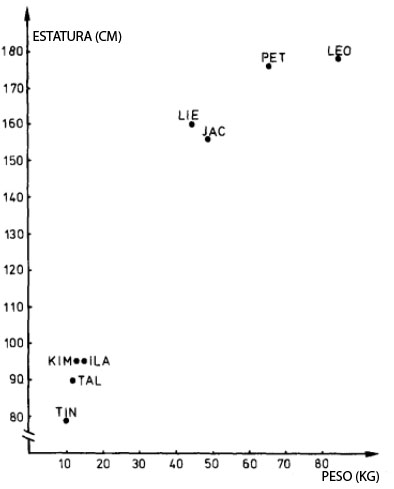
\includegraphics[width=0.5\textwidth]{images/clustering_example.jpg}
    \caption{.}
    \label{fig:clustering_example}
\end{figure}

En el pasado los agrupamientos se realizaban generalmente de manera subjetiva, basándose en el juicio y la percepción del observador. Esto es posible de realizar para casos simples con 2 o 3 dimensiones, como el de la figura \ref{fig:clustering_example}, donde se pueden reconocer a simple vista 2 grupos \{ILA, KIM, TIN, TAL\} y \{JAC, LEO, LIE, PET\}. Sin embargo, en la vida cotidiana es necesario clasificar objetos con una mayor dimensionalidad y realizar este procedimiento de manera más objetiva. Es por esto que se ha desarrollado el procedimiento automático de clasificación.

Con los años se han desarrollado múltiples algoritmos de clasificación, debido a que no existe una definición general de clúster y de hecho existen muchos tipos: clústers esféricos, clústers lineales, entre otros. Además, cada una de las distintas aplicaciones utilizan diferentes tipos de datos como variables discretas, variables continuas, similitudes y diferencias.

A continuación se presentan los algoritmos de \textit{clustering} utilizados.

\subsection{K-Means}

Este es un método de agrupamiento que tiene por finalidad clasificar un grupo de datos en $k$ grupos, basándose en la distancia que presenta cada dato respecto a un centroide. Este algoritmo fue propuesto por Lloyd en 1957, pero no fue publicado hasta el año 1982 \cite{kmeans}.

Para realizar el agrupamiento el algoritmo realiza iteraciones, en donde lleva a cabo un seguimiento de los centroides de los grupos. Antes de la primera iteración se inicializan los centroides con valores aleatorios. En cada iteración se realizan las siguientes tareas. Primero, para cada punto de los datos se encuentra el centroide más cercano y se asocia a este. Después se reestiman las ubicaciones de los centroides con el centro de masa de sus puntos asociados. Luego se repite el mismo proceso de asignar cada punto al centroide más cercano y reestimar la ubicación de los centroides hasta que estos permanezcan fijos en una iteración o se alcance un número determinado de iteraciones. 

En el algoritmo \ref{alg:kmeans} se muestra el pseudocódigo del algoritmo de agrupamiento descrito.

\begin{algorithm}{}
\caption{K-Means \cite{montresordecentralized}}\label{alg:kmeans}
\begin{algorithmic}[1]
\Require K $\geq$ 1
\ForAll{i $\in$ [1..K]}
\State c$_{i} \gets$ ObtenerPuntoAleatorio()
\EndFor
\Repeat 
\State Set all C$_{i}$ equal to $\emptyset$
\ForAll{item $\in$ S}
\State j $\gets$ argmin$_{i}(\|{\textrm{c}_{i}-\textrm{item}}\|)$
\State C$_{j}$ = C$_{j} \cup \{\textrm{item}\}$
\EndFor
\ForAll{i $\in$ [1..K]}
\State $\textrm{old\_c}_{i} = \textrm{c}_{i}$
\State $\textrm{c}_{i} = \frac{1}{\mid{\textrm{C}_{i}}\mid} \displaystyle\sum_{j \in \textrm{C}_{i}}j$
\EndFor
\Until $\forall_i , \textrm{old\_c}_{i} = \textrm{c}_{i}$
\State \textbf{return} all C$_{i}$
\end{algorithmic}
\end{algorithm}

Las principales ventajas que presenta este algoritmo son: facilidad para ser implementado, simple y general. Por otro lado, sus desventajas son: se debe especificar un $k$, muy sensible a la inicialización de los centroides y su baja escalabilidad. Una mala elección del número de clústers puede repercutir en la obtención de malos resultados, al igual que la inicialización aleatoria de los centroides. Además, mientras más grande es el número de clústers, mayor es la probabilidad de incurrir en mínimos locales.

\subsection{X-Means}

X-Means es un algoritmo de agrupamiento, extendido de K-Means, propuesto por Pelleg y Moore \cite{Pelleg00x-means:extending} el cual busca mejorar la baja escalabilidad computacional, uso de un número determinado de clústers y sensibilidad a mínimos locales.

El principal problema que viene a solucionar este método es el de ingresar con anticipación el número deseado de clústers. A diferencia de K-Means, X-Means recibe un límite inferior y uno superior, dentro del cual el algoritmo es capaz de determinar cual es el número de centroides correcto basándose en una heurística.

El algoritmo \ref{alg:xmeans} generado por Montresor y Guerrieri \cite{montresordecentralized} muestra el funcionamiento de X-Means, el cual está basado en un K-Means reiterativo con $K=2$. Lo que realiza este método es dividir en dos el data set inicial, para luego ir dividiendo en dos cada clúster que se va generando y detenerse cuando el número de clústers es mayor al límite superior.

En palabras sencillas el algoritmo realiza las siguientes operaciones:
\begin{enumerate}
    \item Ejecuta K-Means ($K=2$) en el conjunto completo de datos, tomando dos centroides a partir de un vector aleatorio que pasa por el centro de masa del conjunto original y a una distancia proporcional al tamaño de la región total.
    \item Si los clústers ''hijos'' tienen un desempeño mejor según el criterio de información bayesiano (BIC) que el clúster original, estos se conservan y lo reemplazan. 
    \item Si no existe una mejor representación del clúster original escoge una fracción constante de los clústers y los reemplaza por sus dos ''hijos''.
    \item El algoritmo se detiene cuando el número de clústers es mayor al límite superior entregado al algoritmo.
\end{enumerate}

\begin{algorithm}{}
\caption{X-Means (simplificado) \cite{montresordecentralized}}\label{alg:xmeans}
\begin{algorithmic}[1]
\Require Set de datos S, número máximo de cluster MAX
\Require Función 2Means(S) retorna 2 clústers
\State Clustering $\gets$ 2Means(S)
\State Mejor\_Puntuacion $\gets -\infty$ 
\While{$\mid$Clustering$\mid<$ MAX}
\State Nuevo\_Clustering $\gets$ \{\}
\ForAll{Cl $\in$ Clustering}
\State Cl2 $\gets$ 2Means(Cl)
\If {Medida(Cl) $>$ Medida(Cl2)}
\State Nuevo\_Clustering $\gets$ Nuevo\_Clustering $ \cup $ \{Cl\}
\Else
\State Nuevo\_Clustering $\gets$ Nuevo\_Clustering $ \cup $ Cl2
\EndIf
\EndFor
\State Clustering $\gets$ Nuevo\_Clustering
\If {Measure(Clustering) $>$ Mejor\_Puntuacion}
\State Mejor\_Puntuacion $\gets$ Medida(Clustering)
\State Mejor\_Clustering $\gets$ Clustering
\EndIf
\EndWhile\label{euclidendwhile}
\State \textbf{return} Mejor\_Clustering %\Comment{The gcd is b}
\end{algorithmic}
\end{algorithm}

Lo anteriormente descrito se puede apreciar de forma gráfica en la figura \ref{f:xmeans_steps}, donde se encuentra una representación para una iteración del algoritmo, con un conjunto inicial de 3 clústers.

\begin{figure}[H]
 \centering
  \subfloat[El resultado de ejecutar K-Means con 3 centroides.\label{fig:xmeans-1}]{
   \label{f:step1}
    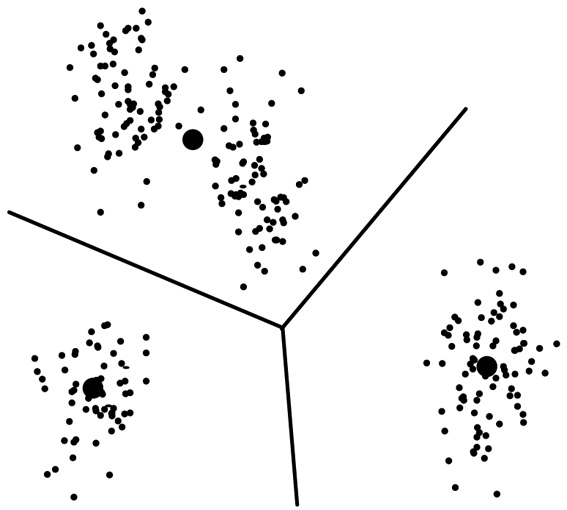
\includegraphics[width=6cm]{images/xmeans1.jpg}}\vspace{1mm}
  \subfloat[Cada centroide original se divide en dos hijos.\label{fig:xmeans-2}]{
   \label{f:step2}
    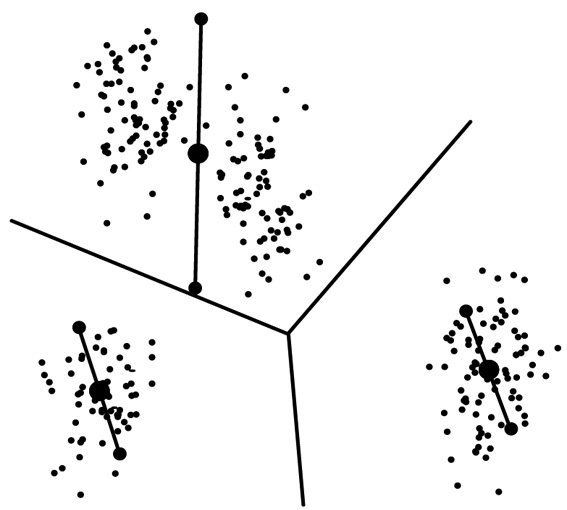
\includegraphics[width=6cm]{images/xmeans2.jpg}}\hspace{1mm}
  \subfloat[El resultado después de que todos los 2-Means paralelos hayan terminado.\label{fig:xmeans-3}]{
   \label{f:step3}
    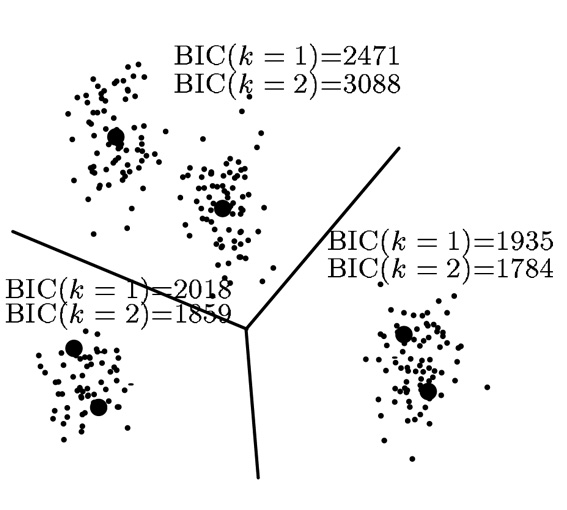
\includegraphics[width=6cm]{images/xmeans3.jpg}}\vspace{1mm}
  \subfloat[Los centroides sobrevivientes después de todas las pruebas de puntuación.\label{fig:xmeans-4}]{
   \label{f:step4}
    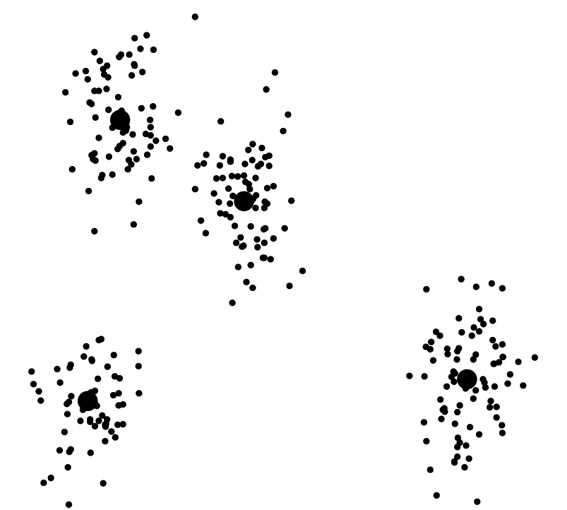
\includegraphics[width=6cm]{images/xmeans4.jpg}}
 \caption{Iteración X-Means.}
 \label{f:xmeans_steps}
\end{figure}

En la figura \ref{fig:xmeans-1} se muestra una solución de K-Means con 3 centroides y los límites de cada región. En la \ref{fig:xmeans-2} se dividen los centroides en dos nodos hijos, trazando un vector aleatorio a una distancia proporcional al tamaño de la región. Luego de esto se ejecuta un K-Means con $k = 2$ de manera local, esto debido a que los hijos solo se distribuyen los puntos de los padres y no se relacionan con el resto. El resultado al finalizar los K-Means se muestra en la figura \ref{fig:xmeans-3}, donde cada hijo tiene sus puntos asociados.

Una vez finalizado lo anterior es momento de evaluar si el padre o los hijos representan mejor la distribución de cada región. Según este criterio se eliminará el padre o su descendencia. Si la representación original de una región es la adecuada, entonces sobrevivirá el padre y se matará a sus hijos. Por otro lado, las regiones que no estén bien representadas por los centroides recibirán mayor atención, aumentando en ellas el número de centroides. En la figura \ref{fig:xmeans-4} se muestra el resultado final al llevar a cabo la prueba de puntuación (BIC) en los 3 pares de hijos.

Una de las principales ventajas que posee este algoritmo radica en que es más escalable debido a que con cada iteración se reduce más el número de datos en los cuales K-Means se debe ejecutar, lo que hace que sea más fácil utilizarlo en conjuntos de datos de mayor tamaño. Otra ventaja es que se sabe que con K-Means de pocos clústers es menos probable incurrir en mínimos locales en comparación a uno realizado con muchos clústers. Por lo tanto, el hecho de que X-Means utilice un K-Means con $K=2$ favorece a que no se atasque en mínimos locales.

Además este método permite realizar una visualización del tipo árbol, la que crea una estructura jerárquica de los clústers.

El porqué se utilizará este algoritmo es debido a su sencillez y facilidad de implementación y ejecución. Además, otro punto importante por el cual se optó por este algoritmo es porque el problema que se busca resolver cuenta con una gran cantidad de datos, lo que no es una dificultad debido a la escalabilidad que este posee gracias a que con cada iteración el conjunto de puntos sobre el cual se aplica K-Means ($k=2$) se ve reducido. Por último, pero no menos importante, se escogió este algoritmo debido a que no necesita conocer de antemano un número de clústers, sino que es calculado automáticamente.

\subsection{CRISP-DM}

CRISP-DM \cite{Wirth00crisp-dm:towards} (\textit{ Cross Industry Standard Process for Data Mining}) es una de las metodologías que más se utiliza para el desarrollo de proyectos de minería de datos. Esta proporciona una visión general del ciclo de vida de un proyecto de minería de datos. Además contiene las fases de un proyecto, sus respectivas tareas y sus resultados.

Este ciclo esta compuesto por 6 fases que se aprecian en la figura \ref{fig:CRISP-DM_diagrama}. Dentro del diagrama las flechas solo indican las dependencias más importantes y frecuentes entre las fases, en donde la secuencia no es estricta. En la figura \ref{fig:CRISP-DM_diagrama} el círculo exterior representa la naturaleza cíclica de la minería de datos. Este proceso no termina una vez se implemente la solución, debido a que todo lo aprendido durante el proyecto puede desencadenar nuevas preguntas de negocio, en donde dichos procesos se beneficiarán de experiencias anteriores.

\begin{figure}[H]
    \centering
    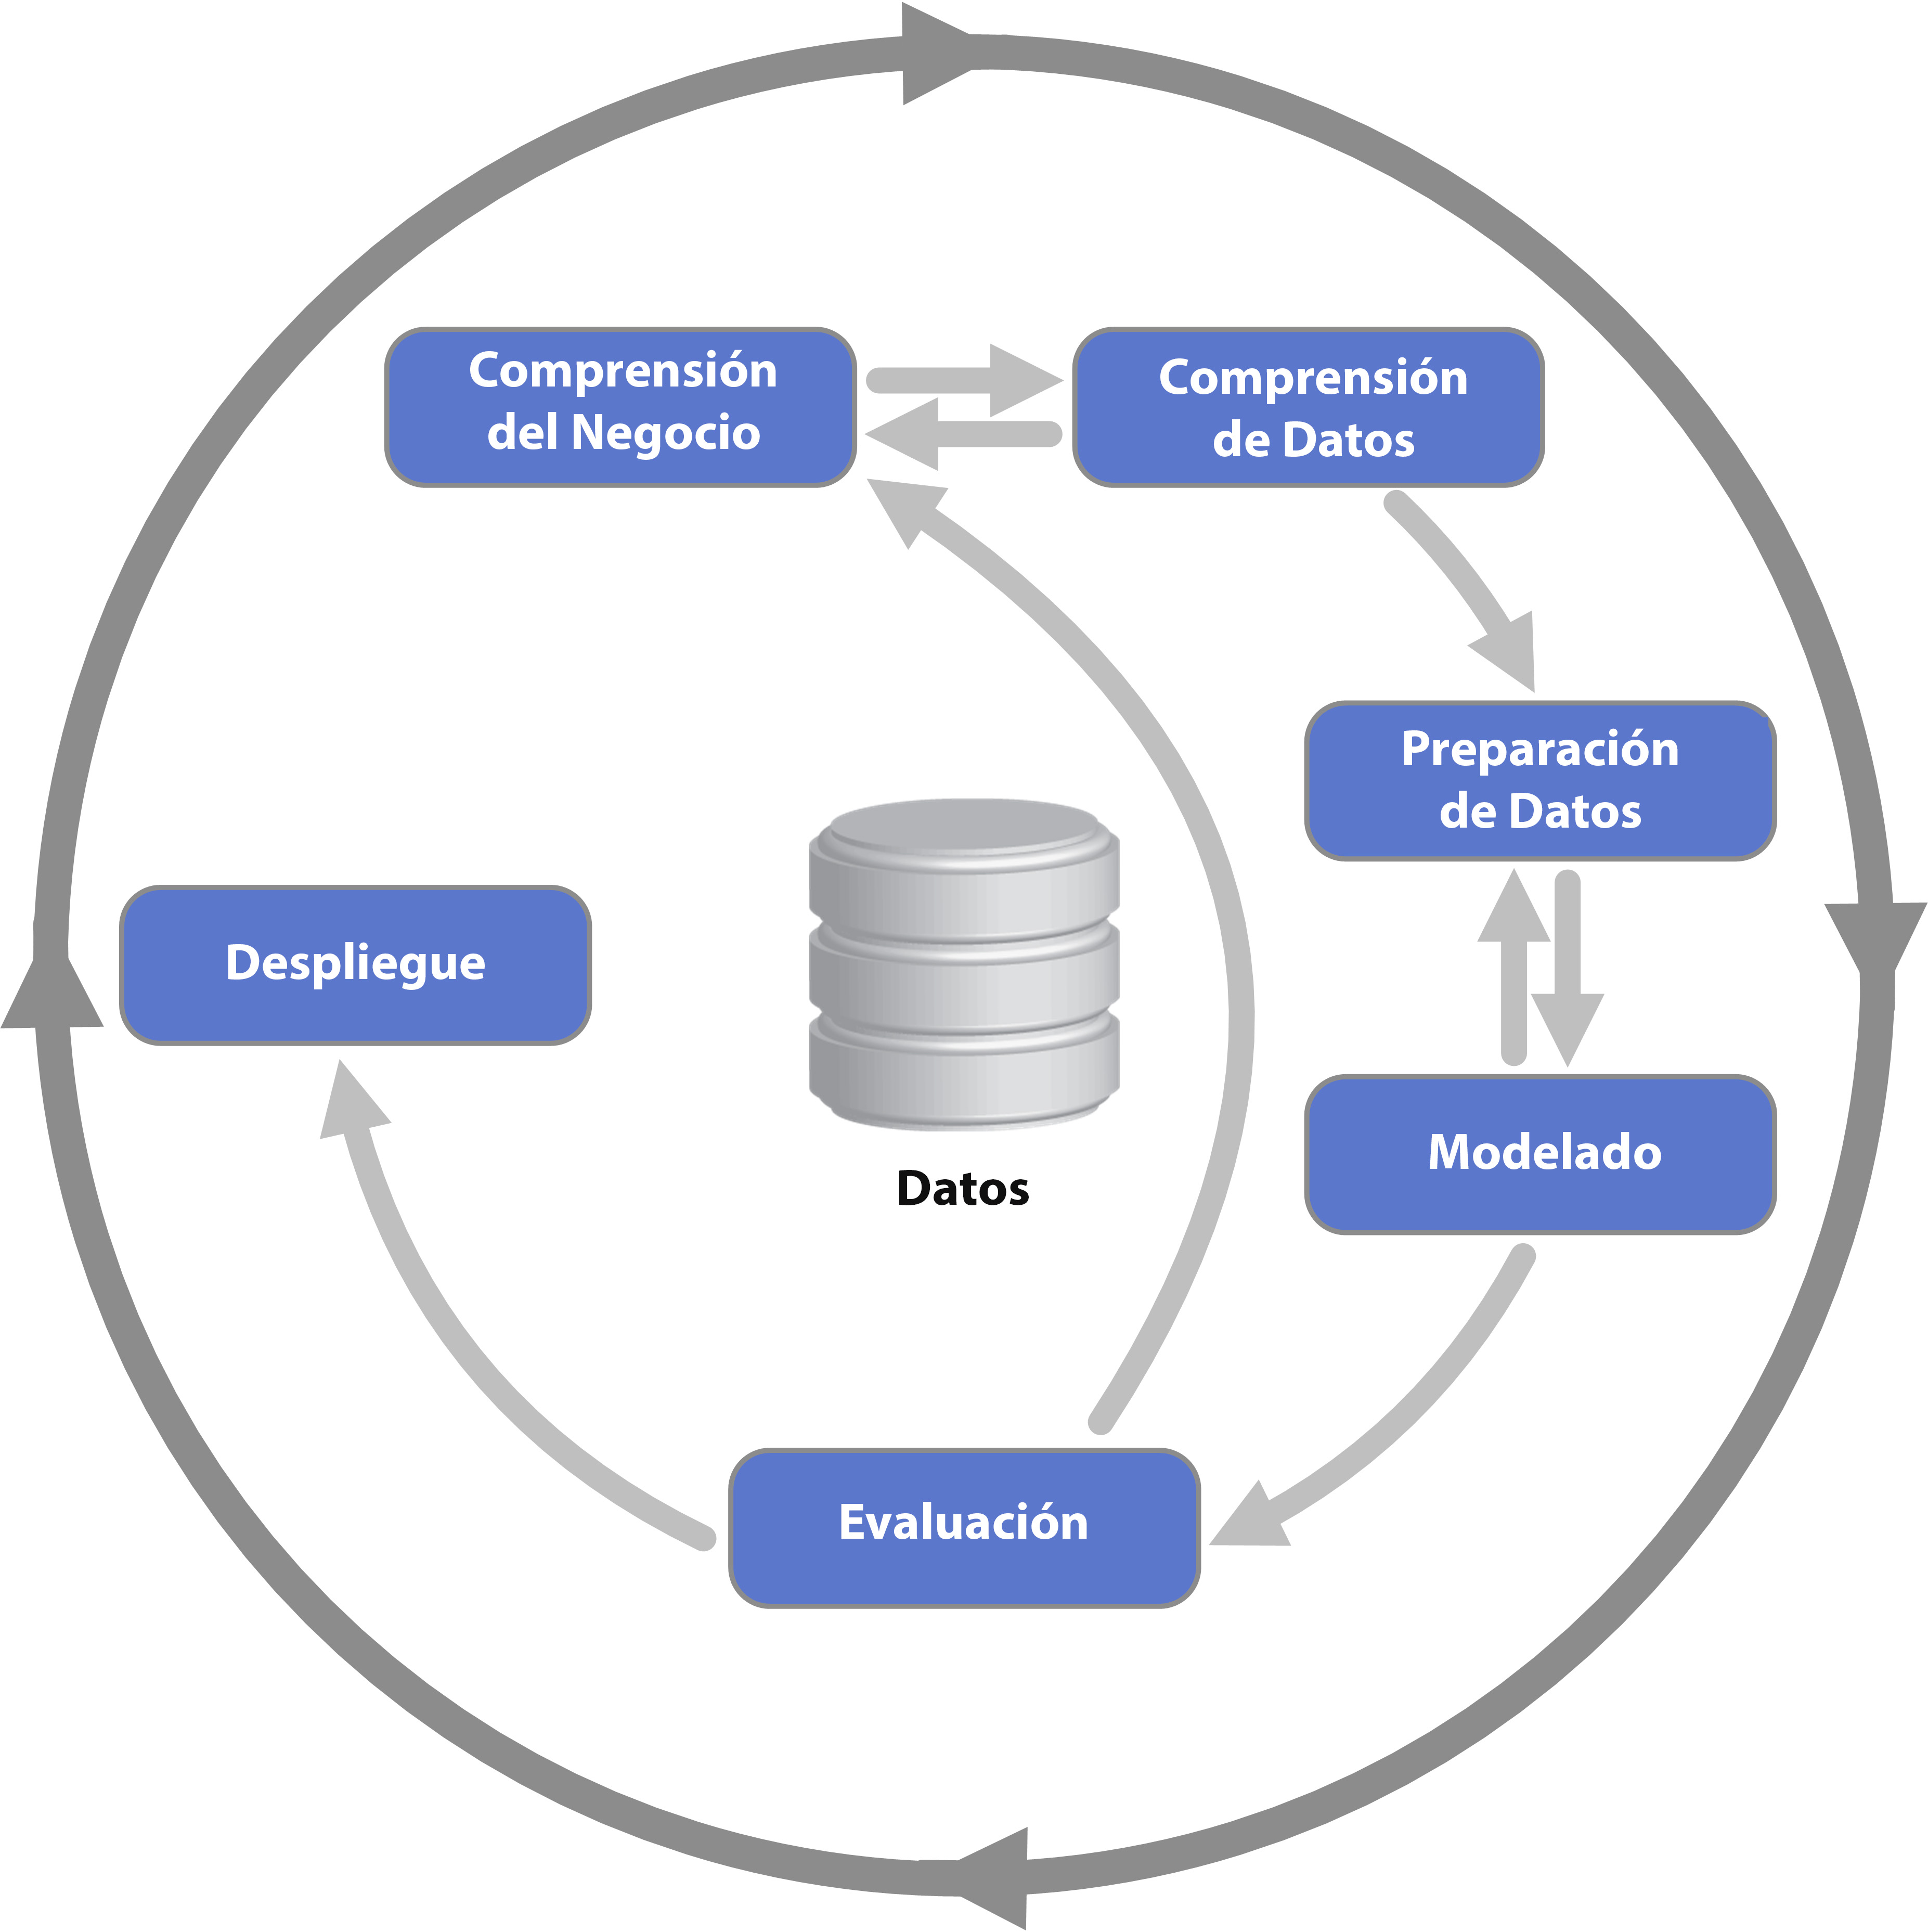
\includegraphics[width=0.5\textwidth]{images/CRISP-DM_Process_Diagram.jpg}
    \caption{Diagrama de proceso que muestra la relación entre las diferentes fases de CRISP-DM.}
    \label{fig:CRISP-DM_diagrama}
\end{figure}

\begin{enumerate}
    \item Comprensión del negocio: Esta fase se centra en comprender los objetivos y requisitos del proyecto desde una perspectiva comercial, para luego convertirlo en una definición del problema de minería de datos. Además, crear un plan preliminar diseñado para alcanzar los objetivos.
    \item Comprensión de datos: Esta fase comienza con una recopilación inicial de datos y actividades para familiarizarse con los datos, identificar problemas de calidad de datos, descubrir primeras ideas sobre los datos o detectar subconjuntos interesantes para formar una hipótesis de información oculta. 
    \item Preparación de datos: Esta cubre todas las actividades para construir el conjunto de datos final a partir de los datos brutos iniciales. Dichas tareas incluyen la selección y transformación de tablas, registros y atributos, construcción de nuevos atributos y limpieza de datos para las herramientas de modelado. Las tareas de preparación de datos puede que se realicen varias veces y sin un orden específico.
    \item Modelado: Fase de selección y aplicación de diversas técnicas de modelado, además de la calibración de sus parámetros para obtener óptimos resultados. Existen varias técnicas para el mismo tipo de problemas de minería de datos. Algunas de ellas requieren formatos de datos específicos.
    \item Evaluación: En esta etapa se ha creado uno o varios modelos que parecen ser de alta calidad. Antes de realizar el despliegue final es importante evaluar más a fondo el modelo y revisar los pasos ejecutados para construirlo.
    \item Despliegue: En fase se deberá definir como implementar los resultados. Dicha implementación dependerá de los requisitos, esta puede ser tan simple como generar un informe o tan compleja como implementar un proceso repetible de minería de datos.
\end{enumerate}